\documentclass[12pt, letterpaper]{article}
\usepackage[utf8]{inputenc}
\usepackage{amsmath}
\usepackage{changepage}% http://ctan.org/pkg/changepage
\usepackage{titlesec} 
\usepackage{placeins}
\usepackage{caption}
\newcommand\tab[1][1cm]{\hspace*{#1}}
\titleformat{\subsection}[runin]{}{}{}{}[]
\usepackage{graphicx}


\title{CS M148 Homework 3}
\author{Hanna Co}
\date{Due: February 25, 2022}

\begin{document}
\maketitle
\newpage
\section{Multinomial Logistic Regression}
\subsection*{a)} Given $ln\frac{P(Y_i=1)}{P(Y_i=K)} = \beta_iX_i$, we can derive the probability for the event that $Y_i=K$:\\
Since we know the sum of all probabilities must add up to 1:\\
$\sum_{n=1}^{K}P(Y_i=n)=1$\\
$P(Y_i=K)+\sum_{n=1}^{K-1}P(Y_i=n)=1$\\
$P(Y_i=K)+\sum_{n=1}^{K-1}P(Y_i=K)e^{\beta_jX_i}$=1\\
$P(Y_i=K)(1+\sum_{n=1}^{K-1}e^{\beta_jX_i})=1$\\
Thus, the probability for class K is:\\
$P(Y_i=K)=\frac{1}{1+\sum_{n=1}^{K-1}e^{\beta_jX_i}}$\\

\subsection*{b)} We know the prediction for $X_i$ changes from k to r when $P(Y_i=r)>P(Y_i=k)$.\\
From the softmax function, we get that $\frac{e^{\beta_rX_i}}{\sum_{j=1}^{K}\beta_jX_i}>\frac{e^{\beta_kX_i}}{\sum_{j=1}^{K}\beta_jX_i}$\\
This is equivalent to $e^{\beta_rX_i}>e^{\beta_kX_i}$\\
$= \beta_rX_i>\beta_kX_i$\\
$= X_i(\beta_r=\beta_k)>0$\\
This is the decision boundary for two classes $k$ and $r$.

\newpage
\section{Decision Trees}
\subsection*{a)} We first begin by calculating entropy values for the table, and for each split:\\
Total Entropy: $-\frac{5}{11}log_2\frac{5}{11}-\frac{6}{11}log_2\frac{6}{11}=0.994$\\\\
 \begin{tabular}{ |c|c|c| } 
 \hline
 \textbf{Feature} & \textbf{Weighted Average} & \textbf{Info Gain} \\ 
\hline
Price & $\frac{1}{11}[(5(-\frac{3}{5}log_2\frac{3}{5}-\frac{2}{5}log_2\frac{2}{5})) + (4(-\frac{1}{2}log_2\frac{1}{2}-\frac{1}{2}log_2\frac{1}{2})) + 0]$ & 0.1891 \\ 
\hline
Type & 0.9422 & 0.0518 \\ 
\hline
Location & 0.9777 & 0.0163 \\ 
 \hline
Level & 0.9777 & 0.0163 \\ 
 \hline
\end{tabular}\\\\
We split on price, as that gives us the largest entropy gain.\\\\

\textbf{\$ Branch; Entropy = 1}\\
 \begin{tabular}{ |c|c|c| } 
\hline
 \textbf{Feature} & \textbf{Weighted Average} & \textbf{Info Gain} \\ 
\hline
Type & 0.5 & 0.5 \\ 
\hline
Location & 0.5 & 0.5 \\ 
 \hline
Level & 0.5 & 0.5 \\ 
 \hline
\end{tabular}\\\\

\textbf{\$\$ Branch; Entropy = 0.971}\\
 \begin{tabular}{ |c|c|c| } 
\hline
 \textbf{Feature} & \textbf{Weighted Average} & \textbf{Info Gain} \\ 
\hline
Type & 0.8 & 0.171 \\ 
\hline
Location & 0.551 & 0.42 \\ 
 \hline
Level & 0.8 & 0.171 \\ 
 \hline
\end{tabular}\\\\

For the \$\$ branch, splitting on location gives us the largest information gain. As for the \$ branch, the information gain for all feature splits it the same, so we also split on location.\\\\

\textbf{\$/LA Branch; Entropy = 1}\\
 \begin{tabular}{ |c|c|c| } 
\hline
 \textbf{Feature} & \textbf{Weighted Average} & \textbf{Info Gain} \\ 
\hline
Type & 0 & 1 \\ 
\hline
Level & 1 & 0 \\ 
 \hline
\end{tabular}\\\\

\textbf{\$\$/Burbank Branch; Entropy = 0.9183}\\
 \begin{tabular}{ |c|c|c| } 
\hline
 \textbf{Feature} & \textbf{Weighted Average} & \textbf{Info Gain} \\ 
\hline
Type & 0 & 0.9183 \\ 
\hline
Level & 0.6667 & 0.2516 \\ 
 \hline
\end{tabular}\\\\

For both branches, we split on Type, which gives us our final tree:\\
\begin{figure}[h!]
  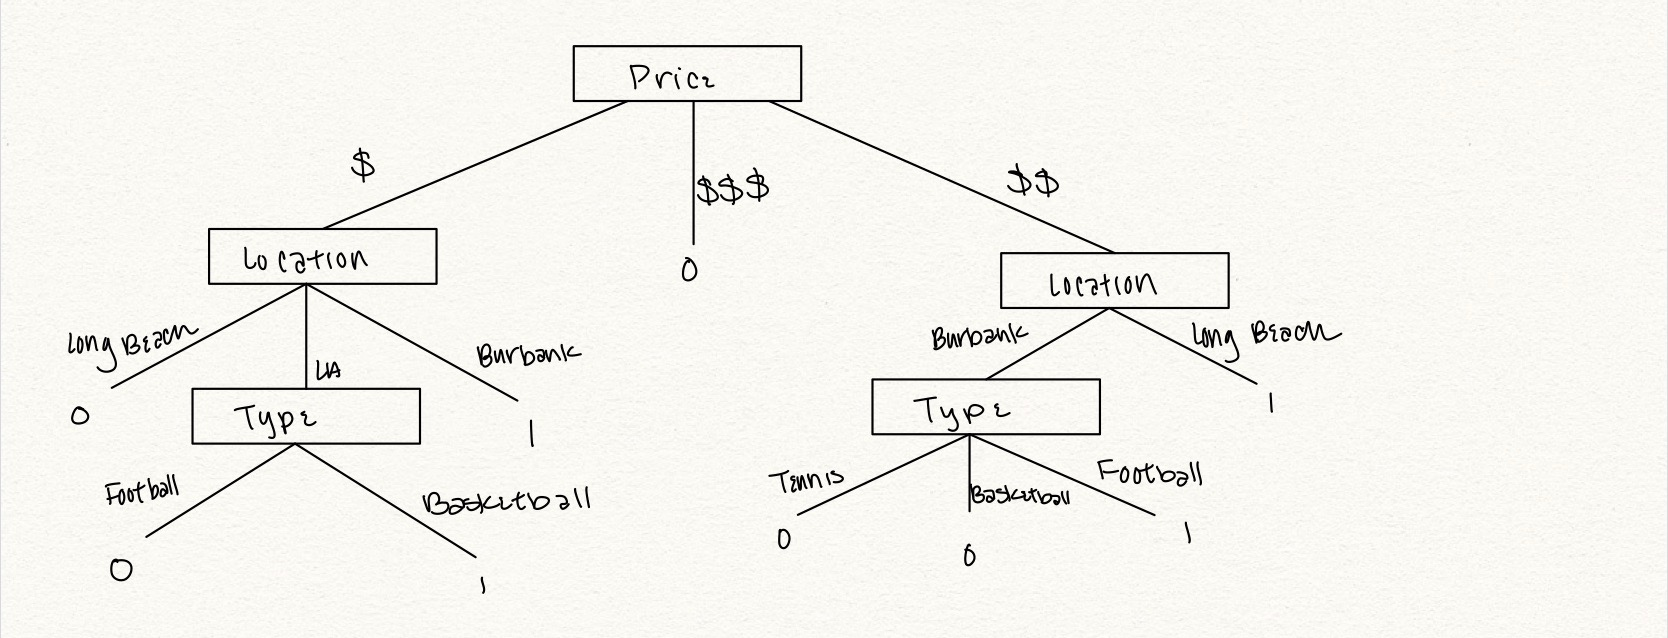
\includegraphics[scale=0.3]{./images/2a}
\end{figure}

\subsection*{b)} Our error is $\frac{0}{11}$; our tree classifies all of our training data correctly.

\subsection*{c)} I would go to matches R12, R13, R16.

\subsection*{d)} Our decision tree did not perform well, with an error of $\frac{3}{5}$, and an F1 score of 0.4.

\subsection*{e)} We prune our tree of obtain a more cost-effective tree.\\
 \begin{tabular}{ |c|c|c|c| } 
\hline
 \textbf{Tree} & \textbf{Error} & \textbf{Leaves} & \textbf{Objective} \\ 
\hline
Full & 0.6 & 9 & - \\ 
\hline
LA/Type & 0.6 & 8 & 0 \\ 
\hline
Burbank/Type & 0.6 & 6 & 0 \\ 
\hline
\$/Location & 0.2 & 4 & $\frac{0.6-0.2}{2}=0.2$ \\ 
\hline
\$\$/Location & 0.2 & 3 & 0 \\ 
\hline
Price & 0.4 & 1 & $\frac{0.4-0.2}{2}=-0.1$ \\ 
\hline
\end{tabular}\\\\
Our most cost effective tree would have one split, on price.

\newpage
\section{Decision Tree (Short Answers)}
\subsection*{a)} It's more likely to overfit on the linearly separable data on the left. This is because decision trees are better at fitting datasets that can't be separated by a single line, since they take so many variables into consideration. Decision trees are very prone to overfitting because of this, as they will try to find very precise boundaries between the points. Instead, I would use a logistic regression model, which works better on linearly separable data.

\subsection*{b)}There is no need to standardize our data, as decision trees aren't sensitive to the magnitude of variables.

\subsection*{c)}Yes, decision trees are robust to outliers. This is because we split on certain values, such as being greater or less than some value. For example, say we have [1, 2, 3, 1000], and we split on 2. The fact that we have 1000 as an outlier doesn't affect our results.

\newpage
\section{Random Forest}
\subsection*{a)} $R^2=0.664$
\begin{figure}[h!]
  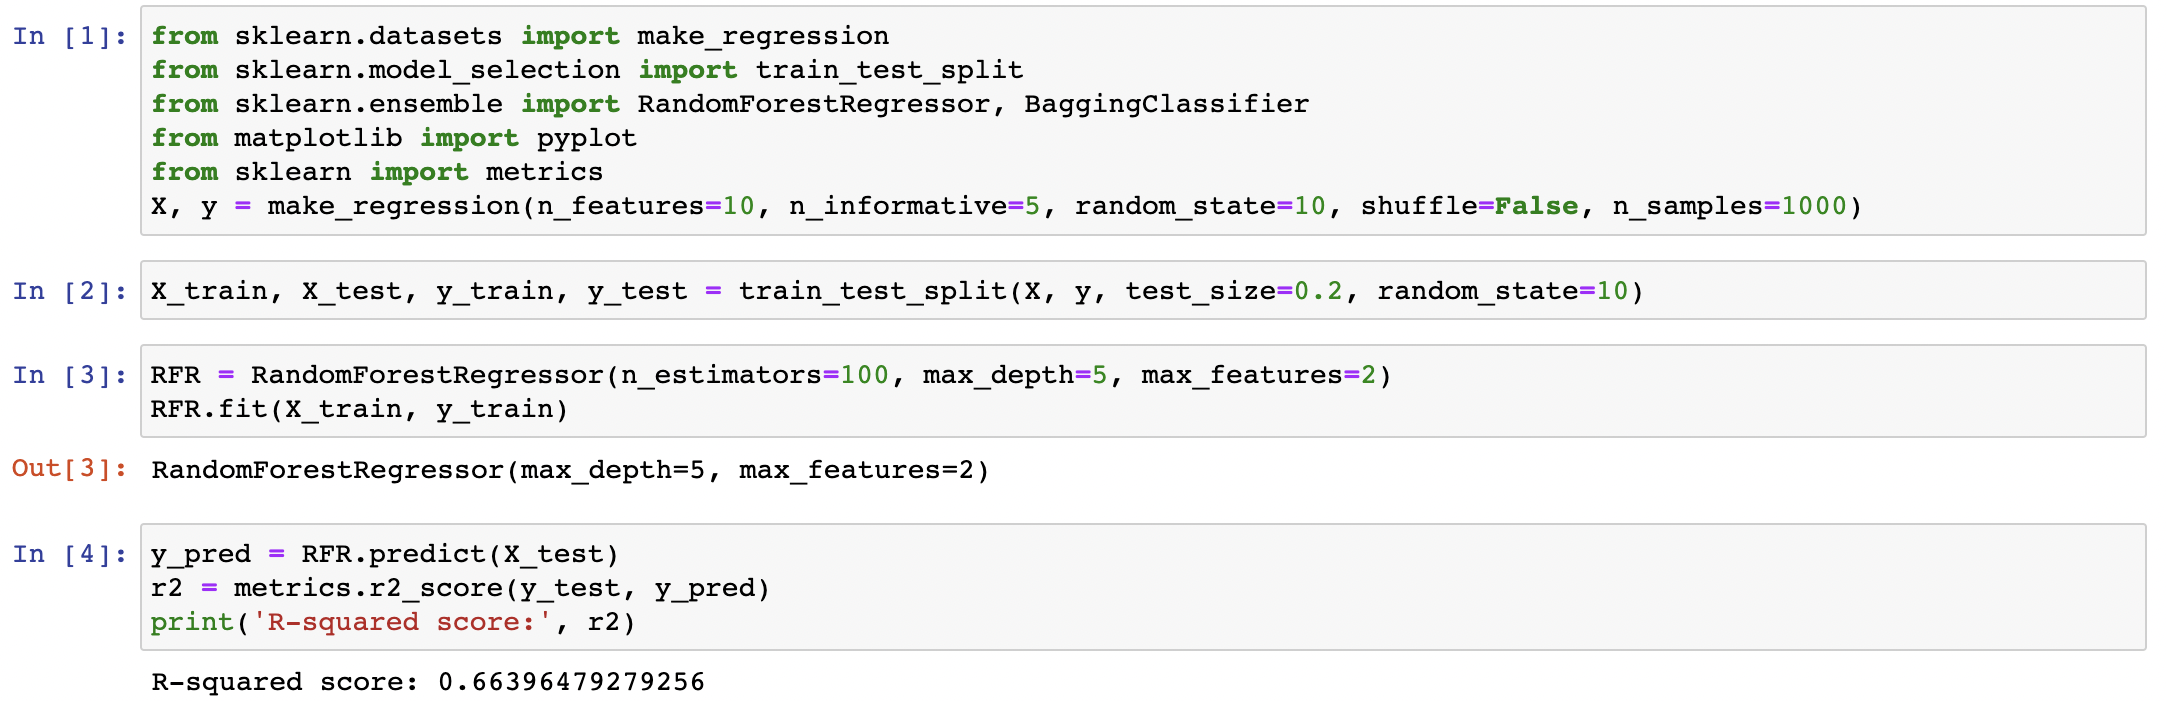
\includegraphics[scale=0.4]{./images/4a}
\end{figure}

\subsection*{b)} To tune the hyperparameters, we use RandomizedSearchCV, and give it some possible parameter values to try and find the best fit. Using this method, I found that the best parameters are \{'n\_estimators': 372, 'max\_features': 'auto', 'max\_depth': 19, 'bootstrap': True\}.\\
\begin{figure}[h!]
  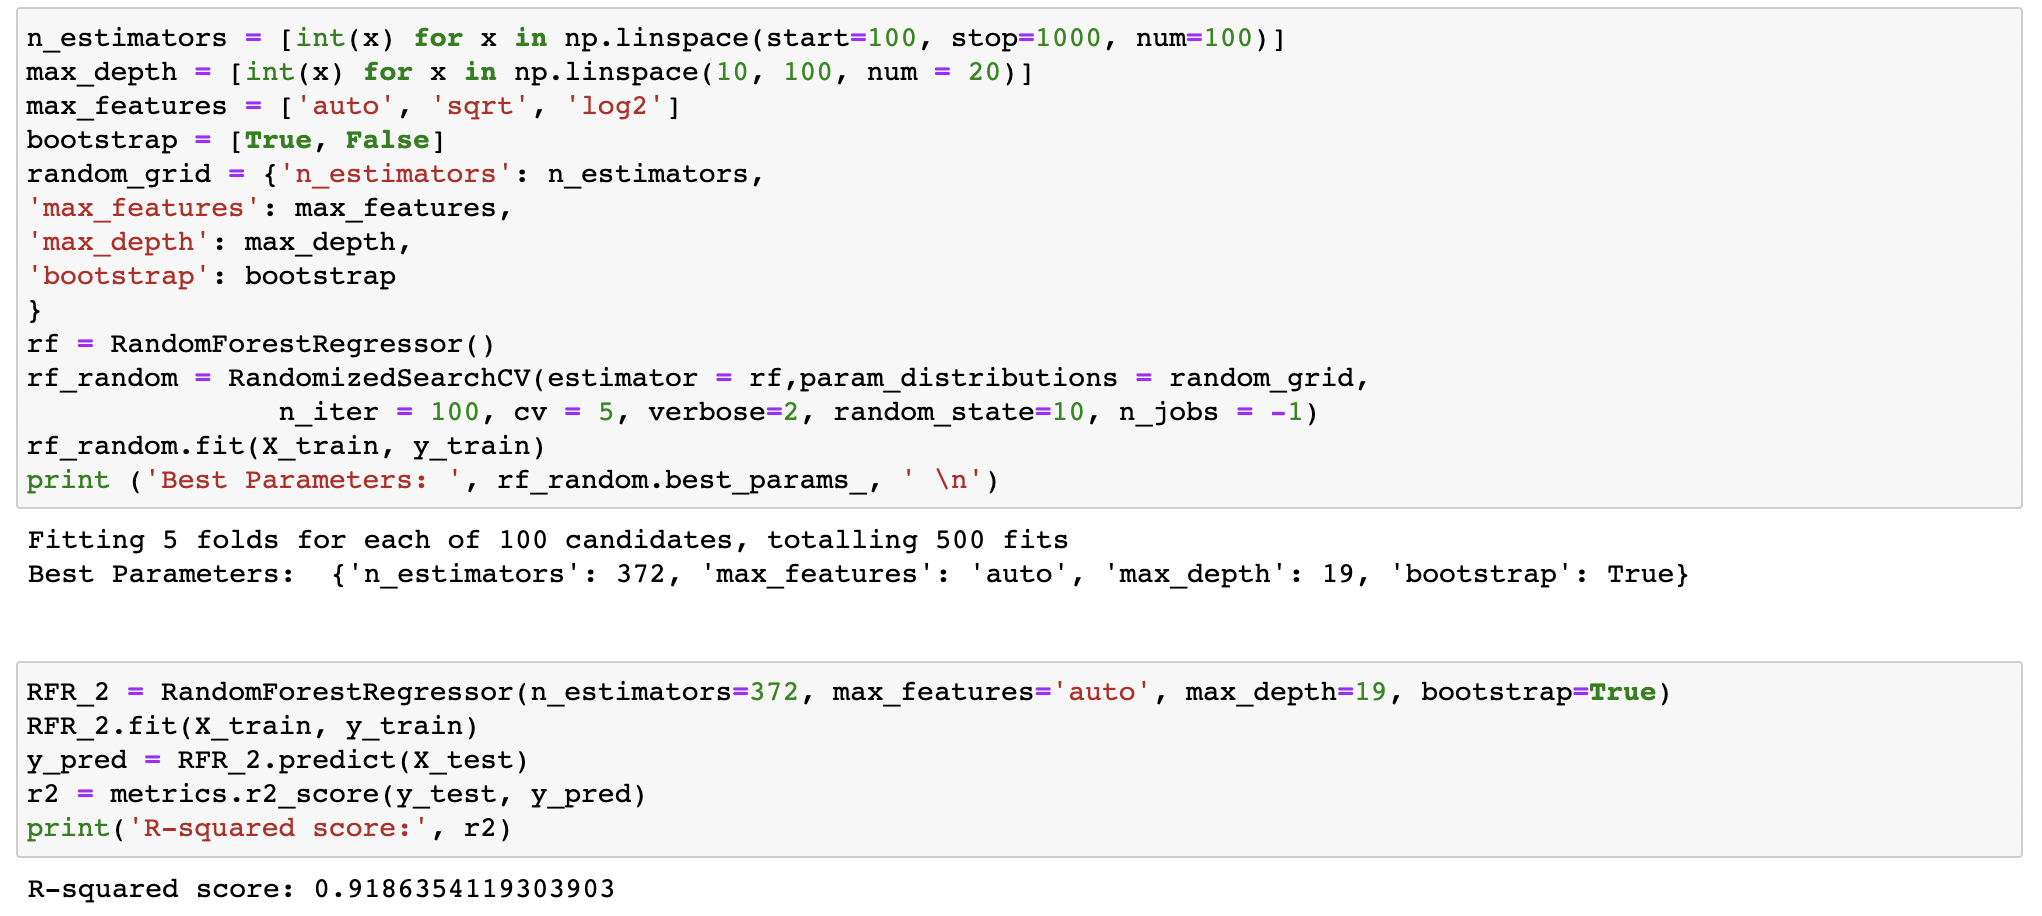
\includegraphics[scale=0.5]{./images/4b}
\end{figure}

\subsection*{c)} Variable Importance
\begin{figure}[h!]
  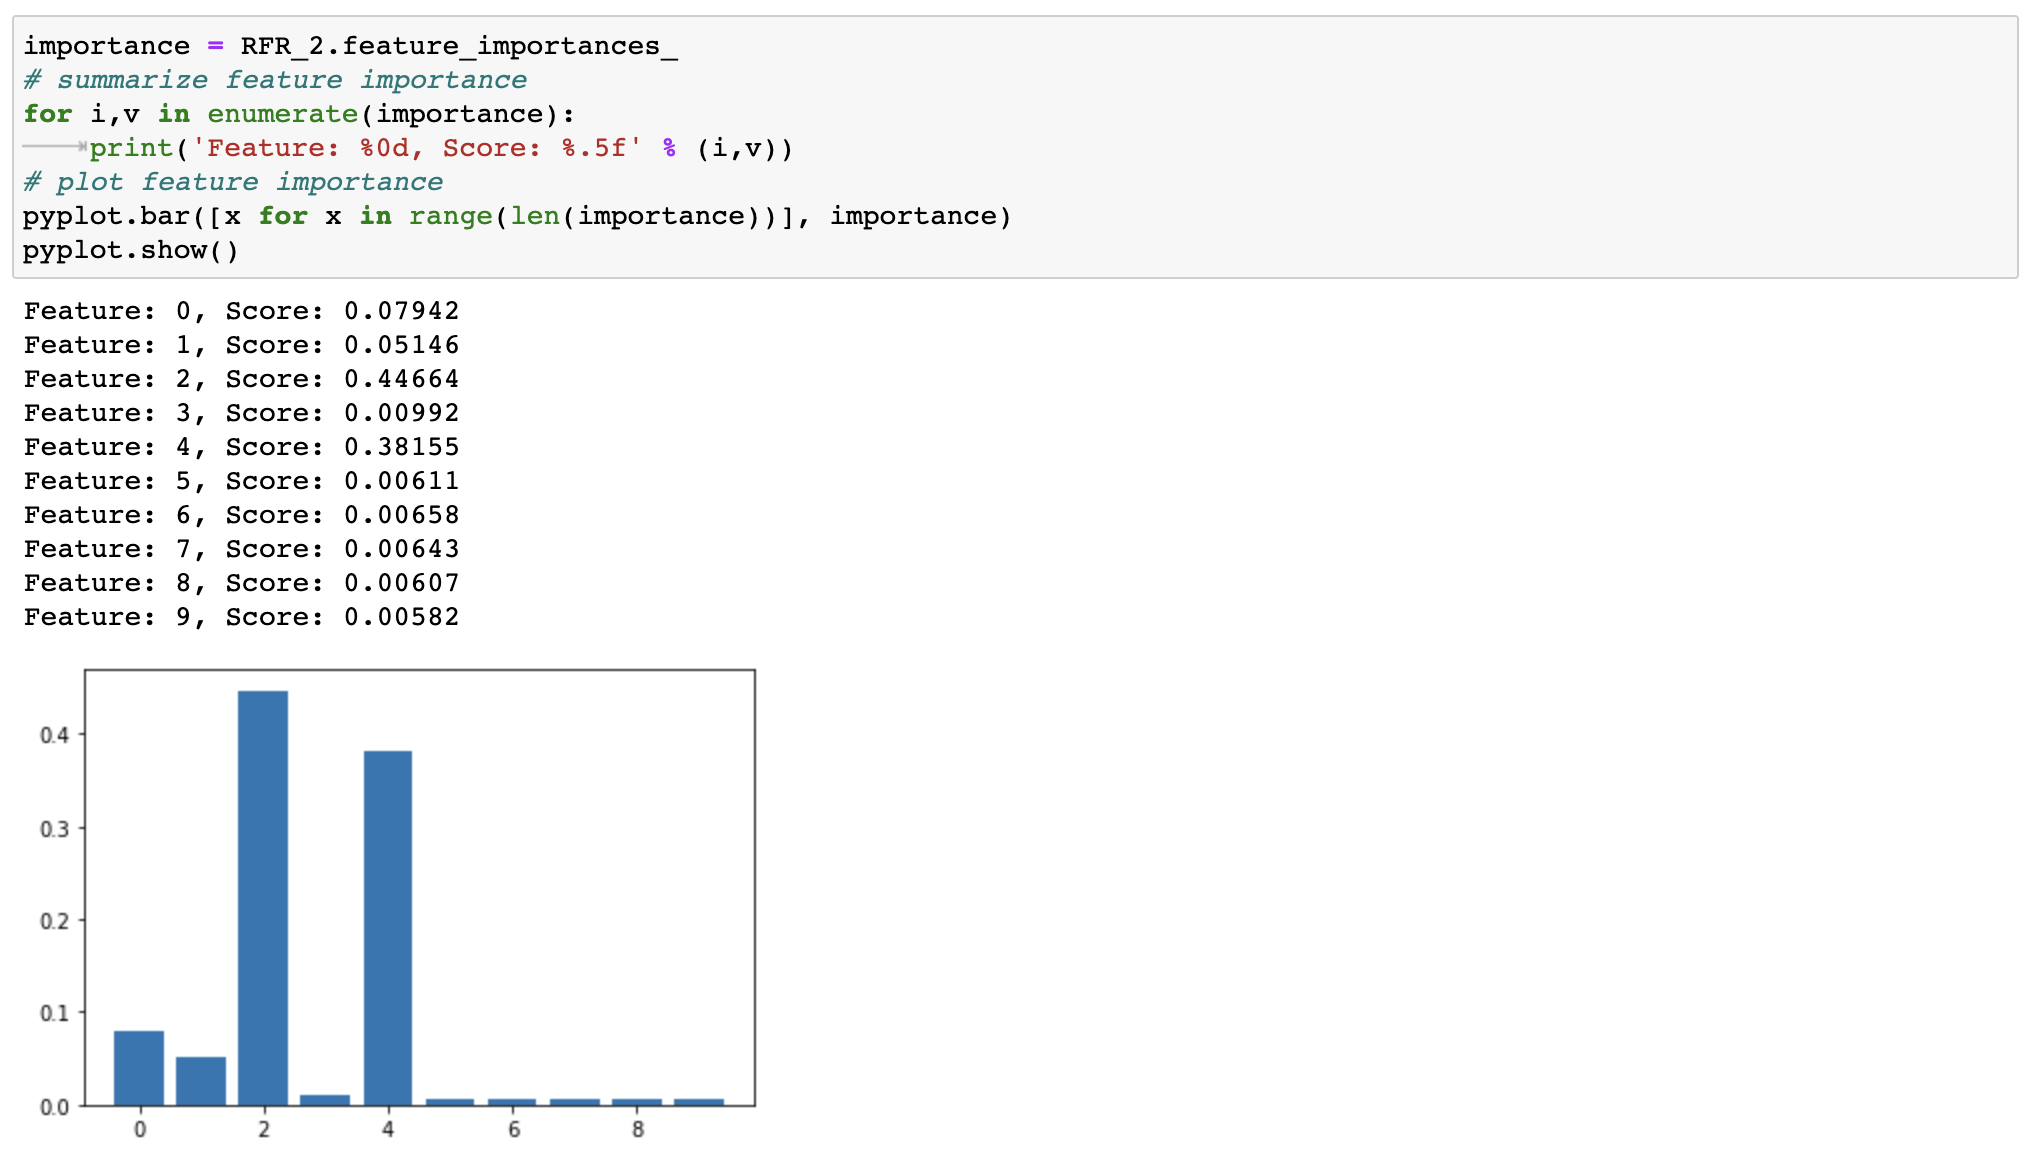
\includegraphics[scale=0.5]{./images/4c}
\end{figure}
\clearpage

\subsection*{d)} As we can see, the feature importance for the two models are nearly identical.
\begin{figure}[h!]
  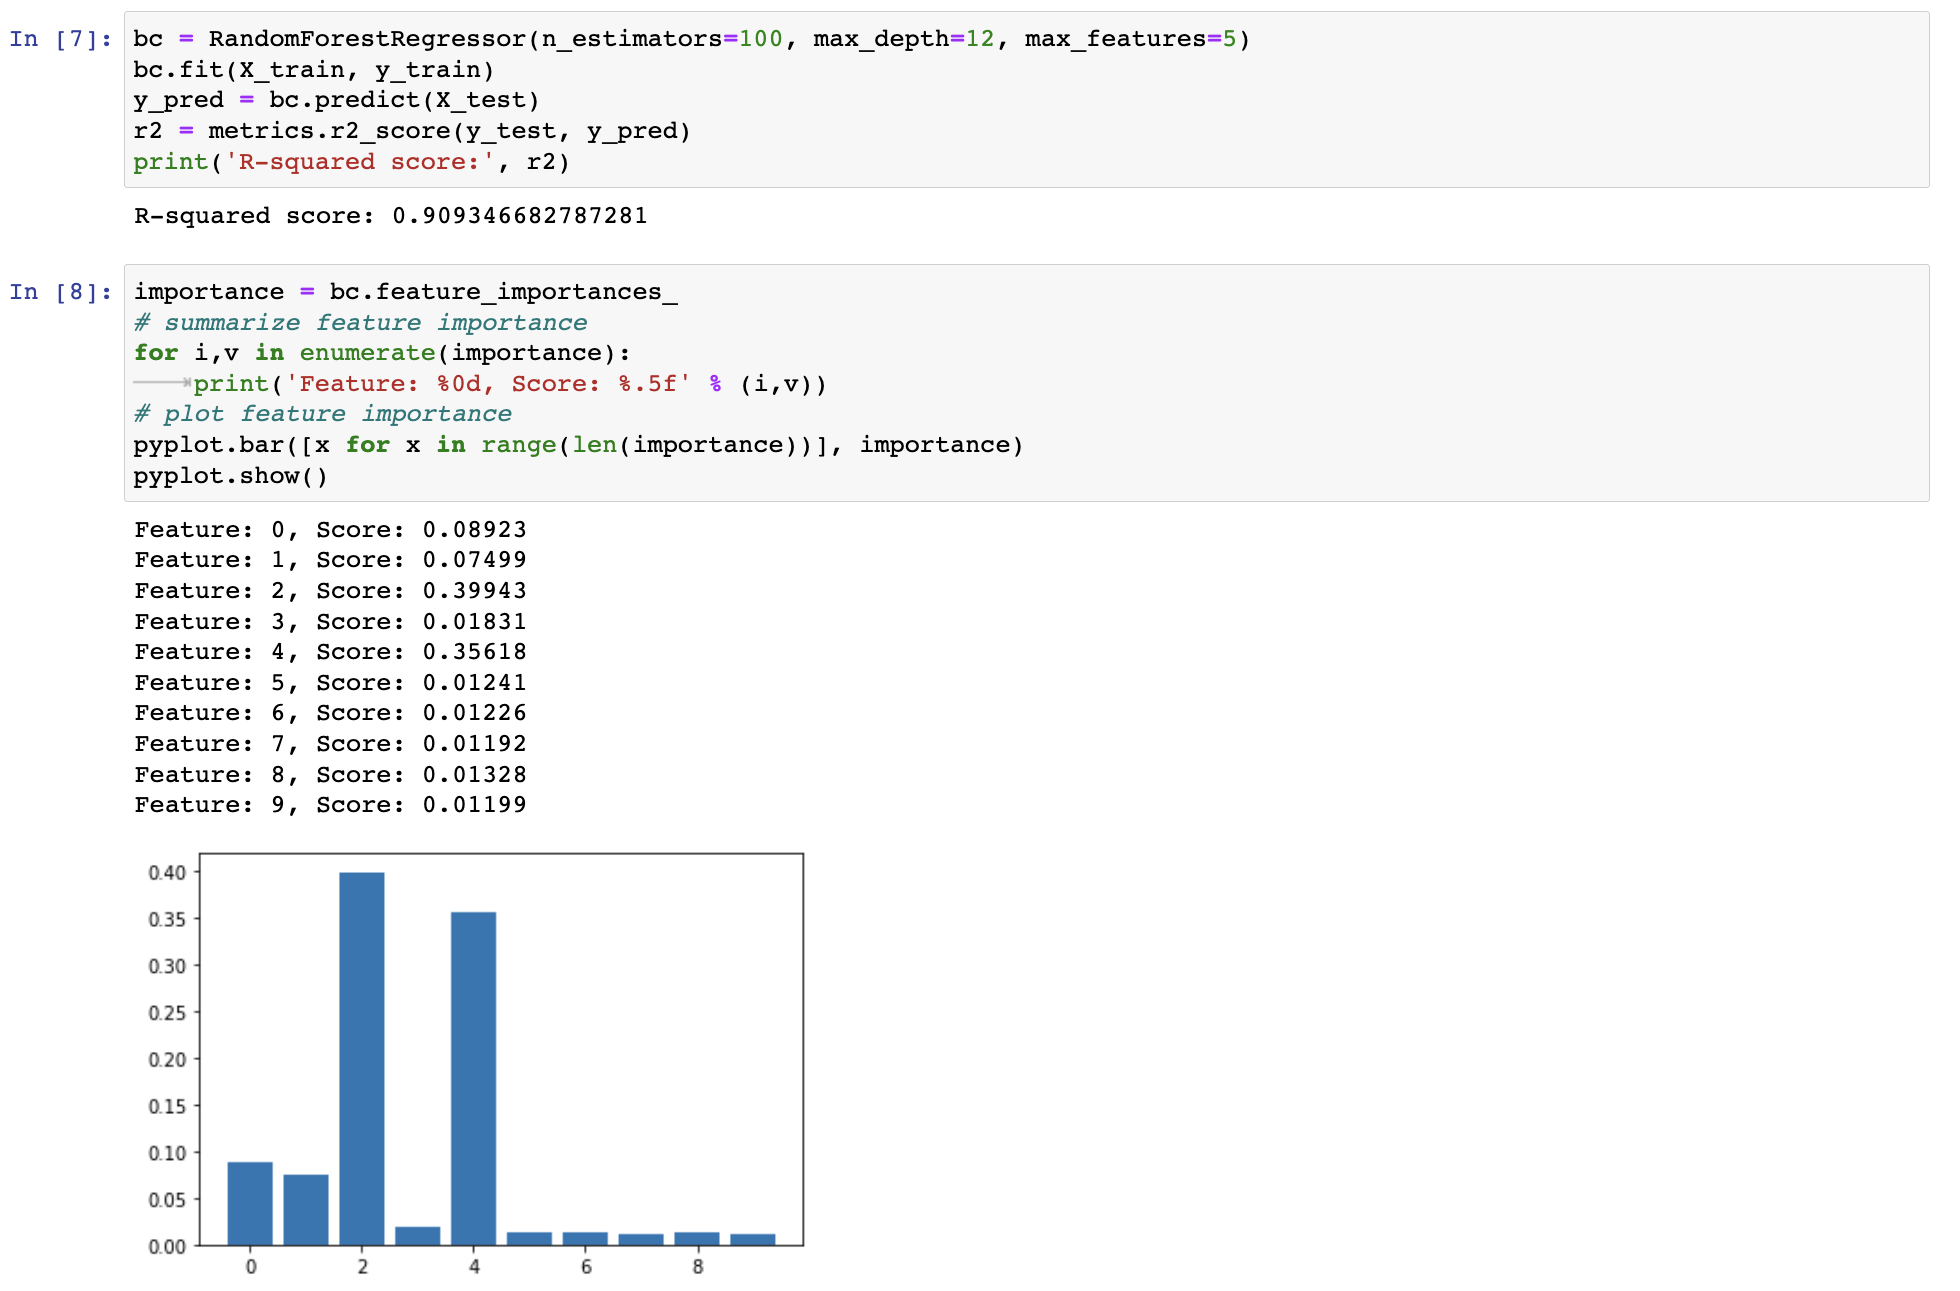
\includegraphics[scale=0.4]{./images/4d}
\end{figure}
\clearpage

\newpage
\section{Perceptron}
\subsection*{a)} $\Delta w_i=x(t-z)*x_i$\\
We are given that $w_1 = w_2 = b = 1$, and $c=2$\\
For the point $(2,-3)$, we can calculate $(2)(1)+(-3)(1)+1 = 0 \Rightarrow 0$\\
Since this does not match our predicted value, we must re-calculate our weights.\\
$\Delta w_1 = 2(1-0)*2 = 4 \Rightarrow w_1 = 1 + 4 = 5$\\
$\Delta w_2 = 2(1-0)*(-3) = -6 \Rightarrow w_2 = 1 - 6 = -5$\\
$\Delta b = 2(1-0)*1 = 2 \Rightarrow b = 1 + 2 = 3$\\
We now make a prediction for our next point, $(4, 4): (4)(5)+(4)(-5)+3 = 3 \Rightarrow 1$\\
Again, this does not match our predicted value, so we mush recalculate our weights.\\
$\Delta w_1 = 2(0-1)*4 = -8 \Rightarrow w_1 = 5 - 8 = -3$\\
$\Delta w_2 = 2(0-1)*4 = -8 \Rightarrow w_2 = -5 - 8 = -13$\\
$\Delta b = 2(0-1)*3 = -6 \Rightarrow b = 3 - 6 = -3$\\
We finally make a prediction for our last point, $(2, -3): (2)(-3)+(-3)(-13)-3 = 30 \Rightarrow 1$\\
This also doesn't match our actual value, so we adjust our weights one last time:\\
$\Delta w_1 = 2(0-1)*2 = -4 \Rightarrow w_1 = -3 - 4 = -7$\\
$\Delta w_2 = 2(0-1)*(-3) = 6 \Rightarrow w_2 = -13 + 6 = -5$\\
$\Delta b = 2(0-1)*(-3) = 6 \Rightarrow b = -3 + 6 = 3$\\

\subsection*{b)} It hasn't converged, because it is still misclassifying points in our data. In this case, I don't expect it to converge, because (2, -3) has both 0 and 1 as actual values, which will continue to confuse our model.

\newpage
\section{ Neural Networks}
\subsection*{a)} Say we have $w_1=w_2=-1$, and $b = 1$. This will give us the following predictions:\\
$(0)(-1)+(0)(-1)+1 = 1 \Rightarrow +1$\\
$(0)(-1)+(1)(-1)+1 = 0 \Rightarrow +1$\\
$(1)(-1)+(0)(-1)+1 = 0 \Rightarrow +1$\\
$(1)(-1)+(1)(-1)+1 = -1 \Rightarrow -1$\\
As we can see, our data can be perfectly classfied with a single activation unit.\\

\subsection*{b)} As we can see from plotting the points, the data is no linearly separable, thus we can not perfectly classify it with a single activation unit.
\begin{figure}[h!]
  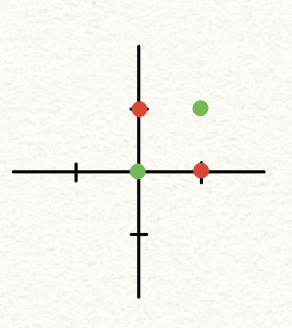
\includegraphics[scale=0.4]{./images/6b.jpeg}
\end{figure}
\clearpage

\subsection*{c)}Yes, you should be able to, by first separating (1, 1) from the other three points, then separating (0, 0) from the other three points. These two activation units and their weights can be combined to form a neural network that perfectly classifies these points.

\newpage
\section{SVM Decision Boundary}
\subsection*{a)} This decision boundary corresponds to plot 4, because it is a linear decision boundary. The support vectors are very close to the boundary, indicating a small C value.

\subsection*{b)} This decision boundary corresponds to plot3, because the decision boundary is linear, with the boundary being far from the support vectors, indicating a large C value.

\subsection*{c)} This boundary corresponds to plot 5, because it is the only quadratic boundary.

\subsection*{d)} This decision boundary corresponds to plot 1, because it is an RBF kernel. It has a smaller $\sigma$ value, so the boundary is tight and well-fitted to the training data.

\subsection*{e)} This decision boundary corresponds to plot 6, because it is an RBF kernel, this time with a large $\sigma$ value, corresponding to a "looser" boundary.


\end{document}